\chapter{Marco Teórico}

\par En este capítulo se presenta un resumen de los conceptos teóricos, modelos matemáticos y algoritmos necesarios para comprender el desarrollo del trabajo y realizar los cálculos que se usaran luego en la sección de metodología.

\par En primer lugar se da una definición de horno de proceso, se explican los tipos de hornos y las secciones generales que componen estos hornos. Luego se describen los métodos de resolución de ecuaciones utilizados. Por último, se elabora sobre las ecuaciones necesarias para simular los fenómenos en cada sección del horno.

\section{Hornos}

\par Un horno de proceso es un equipo constituido por un cerramiento metálico revestido interiormente por una pared refractaria aislante, dentro del cual se dispone de un serpentín tubular por el que circula un producto que se desea calentar y/o evaporar a través del calor liberado por un combustible sólido, líquido o gaseoso que reacciona en el quemador liberando gases de combustión calientes que entregan calor por radiación al serpentín.

\par Un mazo tubular ubicado por encima de de la zona radiante, en el camino de salida de los gases a la chimenea, recupera calor de los humos, mediante un mecanismo de convección. Esta sección se denomina zona convectiva.

\par La utilización de estos equipos puede tener distintos propósitos como precalentamiento de una corriente previo a su fraccionamiento o reacción, evaporar la corriente de fondo de una columna de destilación o disminuir la viscosidad de un fluido para facilitar su manipuleo.
Pueden utilizarse también como reactores, en este caso proveen el calor de reacción. La cantidad de combustible alimentado al horno se regula normalmente en función de la temperatura de salida de la corriente de proceso.

\par Pueden ser considerados intercambiadores de calor en los que el fluido de proceso fluye dentro de tubos y se calienta por radiación procedente de una llama de combustión y por convección desde los gases calientes de esta.

\par Los hornos son definidos en función de su capacidad de suministro de calor (Duty), medida en millones de Kcal/hora o en millones de Btu/hora. Para la mayoría de los hornos instalados en la industria petrolera, la capacidad suele oscilar entre 10 y 350 MM de Btu/hr. [1]

\section{Tipos de hornos}

\par Los hornos son clasificados dependiendo de su diseño mecánico, como se puede apreciar en la Figura \ref{fig:hornos_tipos} las seis clasificaciones b\'asicas son las siguientes:

\begin{enumerate}[label=\Alph*]
    \item .-  Hornos tipo cabina con serpentín albor.
    \item .-  Hornos tipo cilíndrico con serpentín helicoidal.
    \item .-  Hornos tipo cabina con serpentín horizontal.
    \item .-  Hornos tipo cabina doble con serpentines verticales.
    \item .-  Hornos tipo cilíndrico con serpentines verticales.
    \item .-  Hornos tipo cabina doble con serpentines horizontales.
\end{enumerate}

\begin{figure}[hbt]
\begin{center}
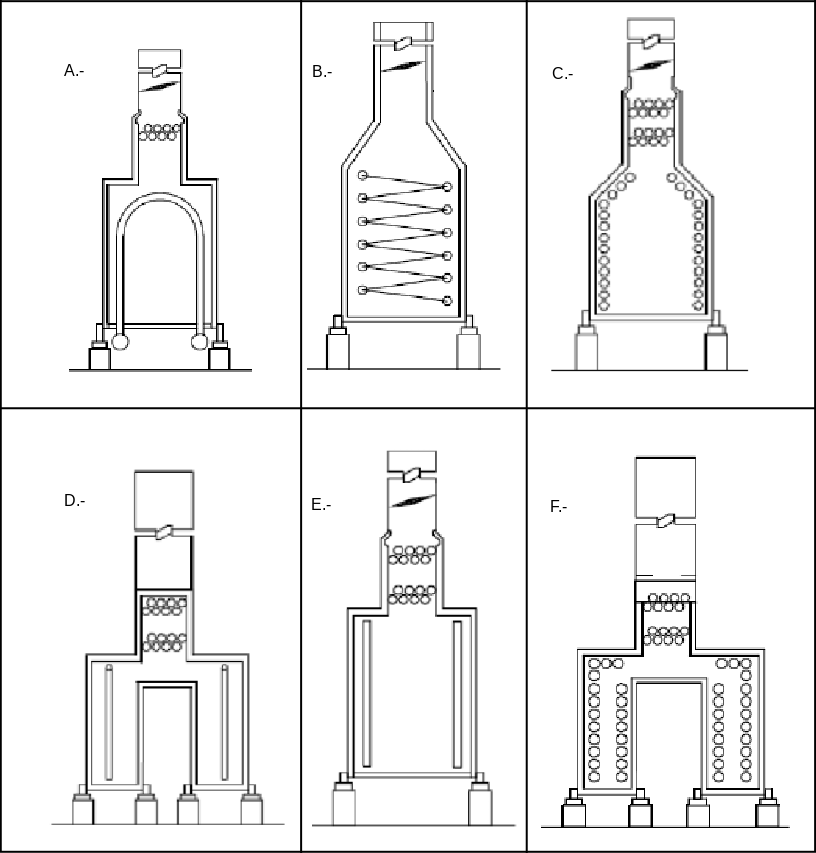
\includegraphics[scale=0.45]{images/hornos_tipos}
\caption[Tipos de hornos por diseño mecánico]{Clasificación de de hornos según su diseño mecánico.}
\label{fig:hornos_tipos}
\end{center}
\end{figure}

\par El horno escogido para simular en este proyecto ha sido uno de tipo cabina con serpentín horizontal, descrito en la Figura \ref{fig:diagrama-meca} y tomado de referencia un horno real ubicado en una refinería de Venezuela.

\begin{figure}[hbt]
\begin{center}
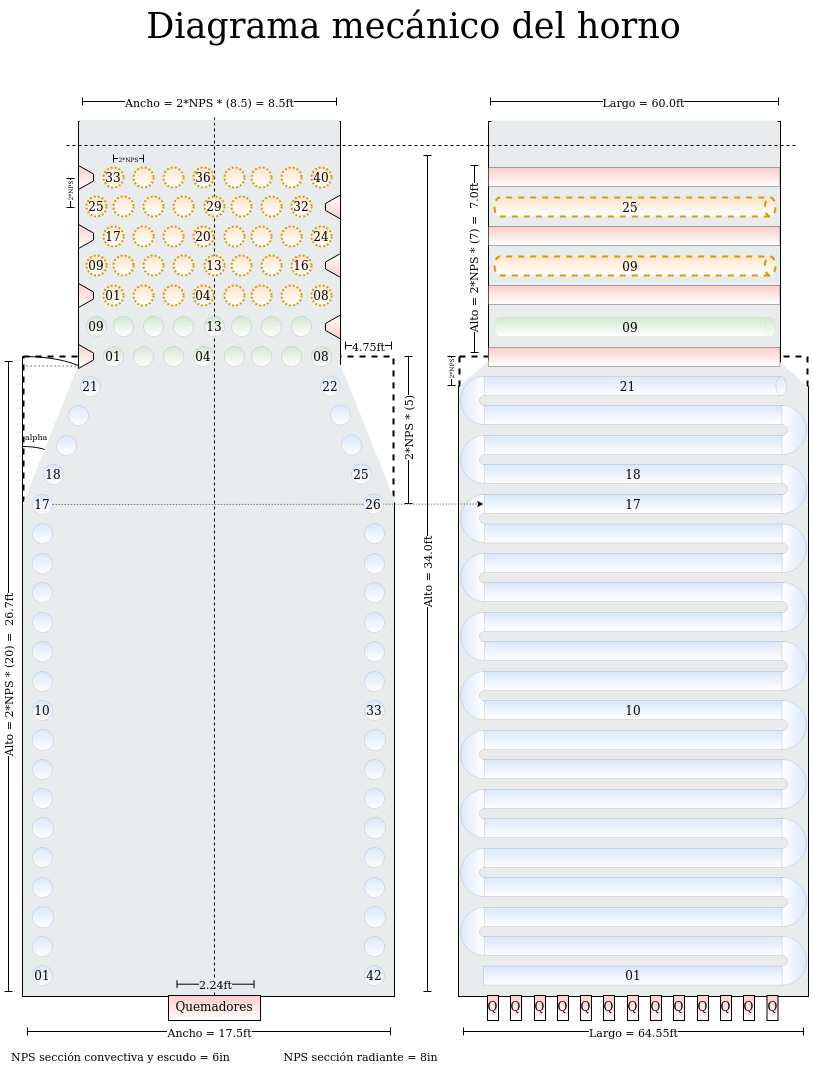
\includegraphics[scale=0.38]{images/diagrama-meca}
\caption[Diagrama mecánico]{Diagrama mecánico del horno simulado.}
\label{fig:diagrama-meca}
\end{center}
\end{figure}

\section{Zonas de un horno}

\par El horno puede ser dividido en zonas o secciones para simplificar los cálculos, como se pudo apreciar en la sección anterior, el arreglo mecánico puede variar pero estas cuatro zonas descritas a continuación son usadas para representar los fenómenos de transferencia de calor internos.

\subsection{Combustión}
\par En esta zona se produce todo el calor usado por el horno para transferir a el fluido ingresado. Este calor proviene de la reacción química de combustión del combustible seleccionado para el proceso.

\par Físicamente seria el espacio donde se mezcla el combustible con el comburente, Oxígeno ($O_2$),
normalmente extraído de una corriente de aire ambiental, cuya composición se aproxima a 20.95\% de ($O_2$) y 79.05\% de Nitrógeno ($N_2$) para los cálculos necesarios. Como ejemplo de esta reacción balanceada se puede observar la ecuación \ref{eq:combustion}, donde se usa Metano ($CH_4$) como combustible, los moles de $N_2$ provienen de la relación volumétrica entre los compuestos del aire teórico 79.05/20.95 = 3.76.

\begin{equation}
    \label{eq:combustion}
    CH_4 + 2O_2 + 2(3.76)N_2 \rightarrow CO_2 + 2H_2O + 7.52N_2
\end{equation}

\par La mínima cantidad de aire que puede suministrar $O_2$ suficiente para una reacción completa es llamado aire teórico. En la practica, la combustión completa no sera lograda a menos que el aire suministrado sea mayor al 100\% del aire teórico y empieza a ser llamado exceso de aire.

\par Un parámetro importante, usualmente usado para expresar la relación de aire y combustible es la relación aire/combustible (designada como AC, ec. \ref{eq:ac}). Usualmente expresada en base másica, pero puedo encontrarse en base molar, como se muestra en la ecuación \ref{eq:ac}

\begin{gather}
    \label{eq:ac}
    AC_{mass} = \frac{m_{aire}}{m_{combustible}}\\
    AC_{molar} = \frac{n_{aire}}{n_{combustible}}
\end{gather}

\par Y se relacionan a través de la masa molar:

\begin{equation}
    AC_{mass} = \frac{m_{aire}}{m_{combustible}} =
    \frac{n_{aire}*M_{aire}}{n_{combustible}*M_{*M_{aire}}} = AC_{molar}*\frac{M_{aire}}{M_{M_{aire}}}
\end{equation}

\par Para profundizar en este tema y observar las ecuaciones de entalpía y energía interna de combustión usadas se recomienda acudir al texto de fundamentos de termodinámica\cite{bib:vanwylen}, capítulo 15, nombrado en las referencias.

\subsection{Radiación}
\par Es donde los tubos que trasportan el fluido de proceso reciben radiación directa desde la llama del quemador y las paredes refractarias. En esta parte la transmisión de calor es por radiación en un 80\% aproximadamente, y un 20\% por convección de la circulación de gases calientes alrededor de los tubos.

\subsection{Convección}
\par Los tubos están fuera del alcance de la llama. Los gases caliente se direccionan a través del paquete de tubos. El calor transmitido es por radiación del CO2 y H2O en los gases calientes además del calor por convección. Los tubos están equipados con aletas para mejorar las condiciones de transmisión de calor.

\subsection{Escudo}
\par Las primeras filas de tubos del área de convección son la zona de escudo (\textit{shield}) en ella los tubos no tienen aletas, reciben la misma cantidad de calor por ambos mecanismos.

\section{Métodos aproximados}
\par A modo de referencia se describen los métodos utilizados a continuación, ya que serán nombrados mas adelante.

\subsection{Newton Raphson}
\par Es un algoritmo para encontrar aproximaciones de los ceros o raíces de una función real. También puede ser usado para encontrar el máximo o mínimo de una función, encontrando los ceros de su primera derivada, pero nuestro caso de enfoque será el mencionado inicialmente.

\par El método de Newton es un método abierto, en el sentido de que no está garantizada su convergencia global. La única manera de alcanzar la convergencia es seleccionar un valor inicial (semilla) lo suficientemente cercano a la raíz buscada. Así, se ha de comenzar la iteración con un valor razonablemente cercano al cero (también denominado punto de arranque o valor supuesto). La relativa cercanía del punto inicial a la raíz depende mucho de la naturaleza de la propia función; si ésta presenta múltiples puntos de inflexión o pendientes grandes en el entorno de la raíz, entonces las probabilidades de que el algoritmo diverja aumentan, lo cual exige seleccionar un valor supuesto cercano a la raíz. Una vez que se ha hecho esto, el método linealiza la función por la recta tangente en ese valor supuesto. La abscisa en el origen de dicha recta será, según el método, una mejor aproximación de la raíz que el valor anterior. Se realizarán sucesivas iteraciones hasta que el método haya convergido lo suficiente. 

\par Así como el valor inicial, el paso de cada iteración y la tolerancia, todas son variables que se ajustan a conveniencia en este método; los rangos de operación alcanzados por el simulador del horno dependerán en gran medida de estos valores.

\par La implementación usada puede verse en los anexos donde se encuentra el código fuente del simulador.

\subsection{Bisección}

\par Es también un algoritmo de búsqueda de raíces que trabaja dividiendo un intervalo dado a la mitad y seleccionando el subintervalo que tiene la raíz. Suele requerir más iteraciones para alcanzar la tolerancia deseada que el Newton Raphson descrito anteriormente, además de conocer de antemano el intervalo donde se encuentra la raíz deseada, su ventaja es que en funciones continuas se puede garantizar su convergencia.
\par Se basa en el teorema del valor intermedio (TVI), el cual establece que toda función continua $f$ en un intervalo cerrado $[a,b]$ toma todos los valores que se hallan entre $f(a)$ y $f(b)$. 
Esto es que todo valor entre $f(a)$ y $f(b)$ es la imagen de al menos un valor en el intervalo $[a,b]$. En caso de que $f(a)$ y $f(b)$ tengan signos opuestos, el valor cero sería un valor intermedio entre $f(a)$ y $f(b)$, por lo que con certeza existe un  $p\in [a,b]$ que cumple  $f(p)=0$. 
De esta forma, se asegura la existencia de al menos una solución de la ecuación $f(x)=0$.

\subsection{Ecuaciones}

\par En cada sección se usaron diferentes ecuaciones por lo que se desglosan en esa estructura.

\subsection{Combustión}
\subsection{Radiación}
\subsection{Escudo}
\subsection{Convección}